\begin{frame}
    \frametitle{Linear Regression}
    \begin{columns}
        \column{.5\linewidth}
            \begin{itemize}
                \item Task: for the given input $x$ predict the real value output $y = f(x)$ 
                \item Fit a hyperplane to data 
                \item Linear  function: simple, easy to understand.
            \end{itemize}
        \column{.5\linewidth}
            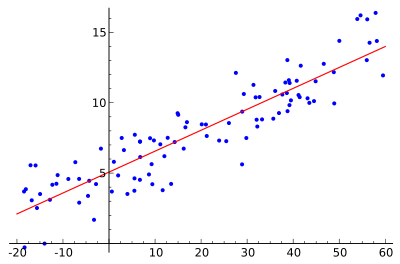
\includegraphics[width=1\linewidth]{linreg-pics/lg2}\\

    \end{columns}
\end{frame}


\begin{frame}
    \frametitle{Example: Okuns Law Quarterly Differences}
    \begin{columns}
        \column{.5\linewidth}
            \begin{itemize}
                \item Data: quarterly change in unemployment rate 
                \item Predict: quarterly change in GDP
            \end{itemize}
        \column{.5\linewidth}
            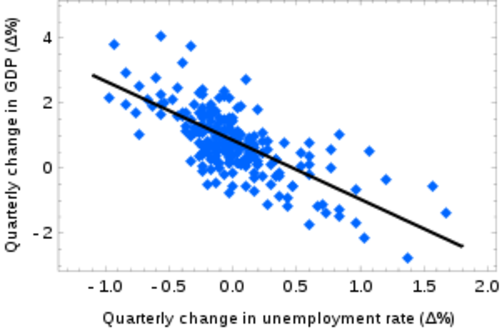
\includegraphics[width=1\linewidth]{linreg-pics/lg}\\

    \end{columns}
\end{frame}


\begin{frame}
    \frametitle{Mathematical Formulation I}
            \begin{itemize}
                \item Linear function: $y =  \left< w, x \right> + b$
                \item $x$ - input vector   
                \item $w$ - weight vector
                \item $b$ - bias
                \item $y$ - output 
            \end{itemize}
\end{frame}


\begin{frame}
    \frametitle{Example for Line}
    \begin{columns}
        \column{.5\linewidth}
            \begin{itemize}
                \item $y =  w_1 x_1 + b$
                \item How do we find coefficients $w_i$ and bias $b$ ? 
            \end{itemize}
        \column{.5\linewidth}
            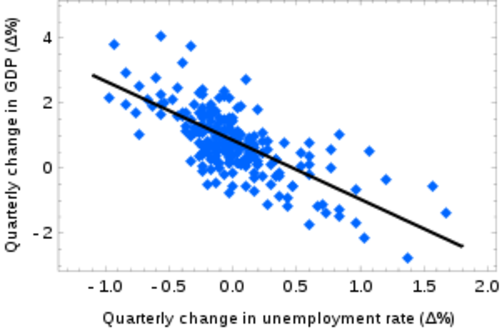
\includegraphics[width=1\linewidth]{linreg-pics/lg}\\

    \end{columns}
\end{frame}





\begin{frame}
    \frametitle{Mathematical Formulation II}
    \begin{columns}
        \column{.5\linewidth}
            \begin{itemize}
                \item Minimize the distance between each data point and the line
                \item $ E = \sum_{i=0}^{N}(y_i - (w_i x_i + b))^2$
                \item Linear regression finds the weights and bias for which the error $E$ is minimal
            \end{itemize}
        \column{.5\linewidth}
            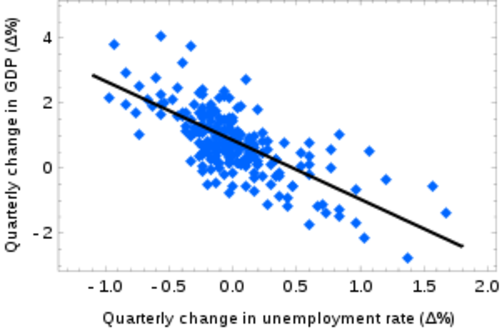
\includegraphics[width=1\linewidth]{linreg-pics/lg}\\
    \end{columns}
\end{frame}


\begin{frame}
    \frametitle{Example: 2D Data}
    \begin{columns}
        \column{.5\linewidth}
            \begin{itemize}
                \item What if our input data has 2-dim?
                \item We can see some linear relationship in the data
            \end{itemize}
        \column{.5\linewidth}
            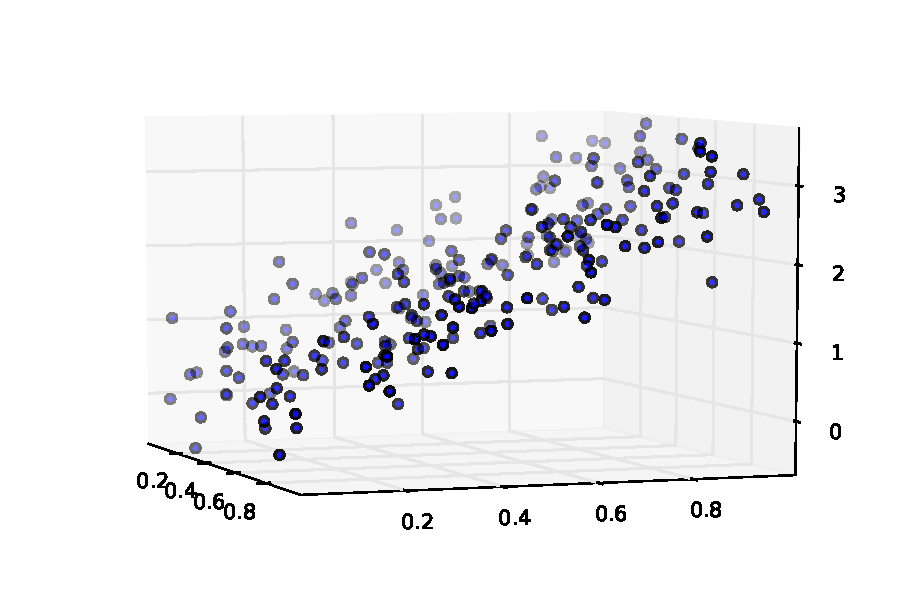
\includegraphics[width=1\linewidth]{linreg-pics/only_data}\\

    \end{columns}
\end{frame}



\begin{frame}
    \frametitle{Example: 2D Data}
    \begin{columns}
        \column{.5\linewidth}
            \begin{itemize}
                \item This time, we are fitting the plane
                \item $y =  w_2 x_2 + w_1 x_1 + b$

            \end{itemize}
        \column{.5\linewidth}
            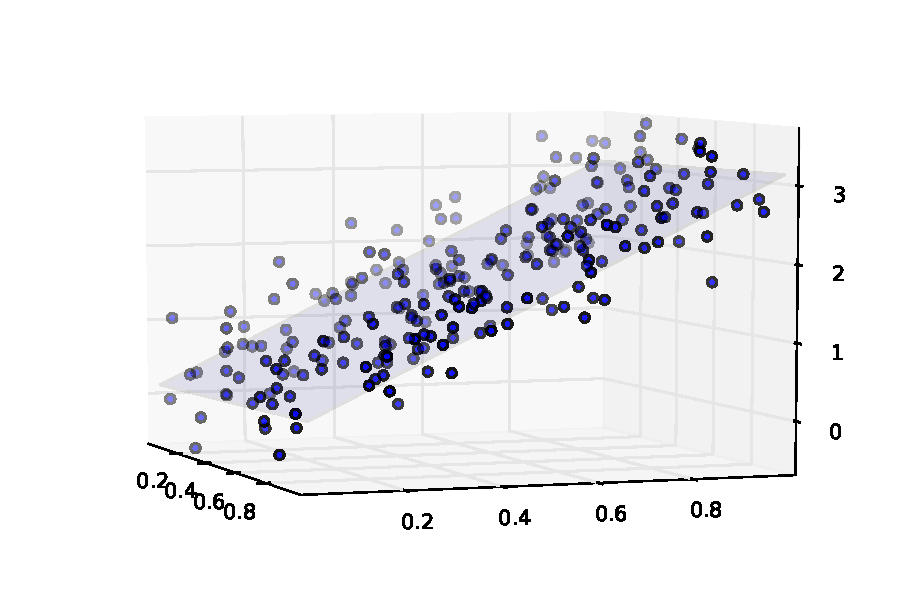
\includegraphics[width=1\linewidth]{linreg-pics/with_plane}\\
            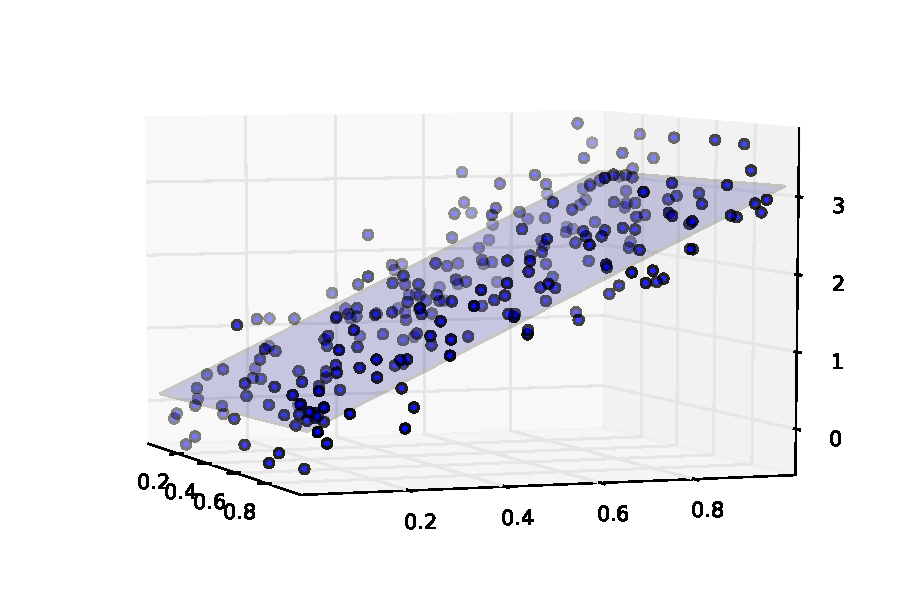
\includegraphics[width=1\linewidth]{linreg-pics/lin_reg_plane}\\

    \end{columns}
\end{frame}


\begin{frame}
    \frametitle{Linear Regression -- Interactive}
    \begin{itemize}
        \item Open Notebook titled 3a - Linear regression 1D.
    \end{itemize}
\end{frame}

